% % % % % % % % % % % % % % % % % % % % % % % % % % % % % % % % % % % % % % % % % % % %
%                                                                                     %
% Short Sectioned Assignment LaTeX Template Version 1.0 (5/5/12)                      %
% This template has been downloaded from: http://www.LaTeXTemplates.com               %
%                                                                                     %
% Original author:  Frits Wenneker (http://www.howtotex.com)                          %
%                                                                                     %
% Modified by: Fco Javier Sueza Rodríguez (fcosueza@disroot.org)                      %
%                                                                                     %
% Changes:                                                                            %
%	    - Custom Chapters, Sections and Subsections (titlesec package)                %
%           - Document type scrbook (oneside)                                         %
%           - Use babel-lang-spanish package and marvosym                             %
%           - Use hyperref, enumitem, tcolorbox and glossaries packages               %
%           - Use Time New Roman (mathptmx), Helvetic and Courier fonts               %
%                                                                                     %
% License: CC BY-NC-SA 3.0 (http://creativecommons.org/licenses/by-nc-sa/3.0/)        %
%                                                                                     %
% % % % % % % % % % % % % % % % % % % % % % % % % % % % % % % % % % % % % % % % % % % %

%-----------------------------------------------%
%	              Packages                  %
%-----------------------------------------------%

\documentclass[paper=a4, fontsize=11pt, oneside]{scrbook}

% ---- Text Input/Output ----- %

\usepackage[T1]{fontenc}
\usepackage[utf8]{inputenc}
\usepackage{mathptmx}
\usepackage[scaled=.92]{helvet}
\usepackage{courier}
\usepackage[indent=12pt]{parskip}

\usepackage{geometry}
\geometry{verbose,tmargin=3cm,bmargin=3cm,lmargin=2.6cm,rmargin=2.6cm}

% ---- Language ----- %

\usepackage[spanish]{babel}
\usepackage{marvosym}

% ---- Another packages ---- %

\usepackage{amsmath,amsfonts,amsthm}
\usepackage{graphics,graphicx}
\usepackage{titlesec}
\usepackage{fancyhdr}
\usepackage{tcolorbox}
\usepackage{hyperref}
\usepackage{enumitem}
\usepackage[automake]{glossaries}

%--------------------------------------------------------------------%
%                      Customizing Document                          %
%--------------------------------------------------------------------%


% ----------- Custom Chapters, Sections and Subsections -------------- %

\titleformat{\chapter}[display]
			{\bfseries\Huge}
			{Tema \ \thechapter} {0.5ex}
			{\vspace{1ex}\centering}

\titleformat{\section}[hang]
			{\bfseries\Large}
			{\thesection}{0.5em}{}

\titleformat{\subsection}[hang]
			{\bfseries\large}
			{\thesubsection}{0.5em}{}

\titleformat{\subsubsection}[hang]
			{\bfseries\large}
			{\thesubsubsection}{0.5em}{}

\hypersetup{
    colorlinks=true,
    linkcolor=black,
    urlcolor=magenta
}

% ------------------- Custom heaaders and footers ------------------- %

\pagestyle{fancyplain}

\fancyhead[]{}
\fancyfoot[L]{}
\fancyfoot[C]{}
\fancyfoot[R]{\thepage}

\renewcommand{\headrulewidth}{0pt} % Remove header underlines
\renewcommand{\footrulewidth}{0pt} % Remove footer underlines

\setlength{\headheight}{13.6pt} % Customize the height of the header

% --------- Numbering equations, figures and tables ----------------- %

\numberwithin{equation}{section} % Number equations within sections
\numberwithin{figure}{section} % Number figures within sections
\numberwithin{table}{section} % Number tables within sections

% ------------------------ New Commands ----------------------------- %

\newcommand{\horrule}[1]{\rule{\linewidth}{#1}} % Create horizontal rule command


%----------------------------------------------------------------------------------------
%	TÍTULO Y DATOS DEL ALUMNO
%----------------------------------------------------------------------------------------

\title{
\vspace{10ex}
\normalfont \normalsize
\huge \textbf{Servicios de Red Implicados en el Despliegue de Aplicaciones}
}
\author{Francisco Javier Sueza Rodríguez}
\date{\normalsize\today}

%----------------------------------------------------------------------------------------
%                                     DOCUMENTO
%----------------------------------------------------------------------------------------
\begin{document}


\maketitle

\thispagestyle{empty}

\vspace{65ex}

\begin{center}
    \begin{tabular}{l l}
        \textbf{Centro}: & IES Aguadulce \\
        \textbf{Ciclo Formativo}: & Desarrollo Aplicaciones Web (Distancia)\\
        \textbf{Asignatura}: & Despliegue de Aplicaciones Web\\
        \textbf{Tema}: & Tema 4 - Servicios de Red Implicados en el Despliegue de Aplicaciones\\
    \end{tabular}
\end{center}

\newpage

\tableofcontents

\newpage

\listoffigures

\newpage

\section{Actividad 1: DNS y Dominio}

\subsection{Enunciado}
\begin{itemize}
    \item \textbf{Actividad 1.1 - Jerarquía de Dominios}: Explica qué son los dominios TLD, cómo se clasifican y pon ejemplos de de varios tipos.
    \item \textbf{Actividad 1.2 - Ventajas del uso de DNS}: Explica las ventajas que aporta el uso de un servicio como el DNS.
    \item \textbf{Actividad 1.3 - Tipo de Registros DNS}: Enumera y explica los tipos de registros DNS más habituales y su finalidad.
    \item \textbf{Actividad 1.4 - Uso del servicio DNS}: Utilizando los comandos vistos en la unidad, averigua la IP a la que responden los siguientes dominios:
    \begin{itemize}
        \item \url{www.educacionfpydeportes.gob.es}
        \item  \url{www.juntadeandalucia.es}
   \end{itemize}
\end{itemize}

\subsection{Solución}

\subsubsection{Jerarquía de Dominios}

    Los \textbf{TLD} (Top Level Domain) o \textbf{Dominios de Nivel Superior} son los dominios al más alto nivel en la jerarquía DNS solo
    después del dominio raíz. Después del dominio raíz, es el primer dominio que se traduce en una dirección IP y representa la última parte del FQDN (Fully Qualified Domain Name) de un dominio, leyéndolos de izquierda a derecha. Estos dominios se pueden clasificar en:
    \begin{itemize}
        \item \textbf{ARPA} (Infrastructura Top-Level Domain): este grupo consiste en un dominio, el \textbf{Addres and Routing Parameter Area} y esta gestionado por el \textbf{IANA} para varios propósitos especificados en los RFC.
        \item \textbf{Dominios TLD Genéricos} (gTLD): están formados por 3 o más letras y se subdividen en:
        \begin{itemize}
            \item \textbf{Dominios de Internet Patrocinados} (sTLD): estos dominios son propuestos y patrocinados por agencias privadas o organizaciones que establecen reglas para poder optar a estos dominios. Algunos ejemplos son: \textbf{edu}, \textbf{gov}, \textbf{int}, etc..
            \item \textbf{Dominios de Internet no Patrocinados} (uTLD): son dominios que no tienen detrás una organización o agencia privada y que imponen menos reglas para su acceso. Algunos ejemplos son: \textbf{com}, \textbf{net}, etc...
        \end{itemize}

        \item \textbf{TLD de Código de País} (ccTLD); estos dominios están asociados con países y territorios y están compuestos por 2 letras.
        Algunos ejemplos son: \textbf{es}, \textbf{us}, \textbf{tk}, etc...
        \item \textbf{TLD de Prueba} (tTLD): estos dominios están instalados bajo \textbf{.test} para la realización de pruebas en el proceso de desarrllo del IDN. Estos dominios no están presentes en la zona raíz.
    \end{itemize}

    Algunos \textbf{ejemplos} de dominios TLD pueden ser los siguientes:

    \begin{itemize}
        \item \textbf{Dominios .info}: destinados principalmente a empresas de información, periódicos, etc..
        \item \textbf{Dominios .es}: destinados a empresas u organizaciones que se encuentran ubicadas en España.
        \item \textbf{Dominios .biz}: proviene de la palabra inglesa \textit{bussines} y esta destinado a empresas y organizaciones con carácter comercial.
        \item \textbf{Dominios .coop}: destinados a cooperativas, siendo necesarios demostrar el carácter de cooperativa a través de organismos locales.
        \item \textbf{Dominios .dev}: destinados a desarrolladores de software.
    \end{itemize}

\subsubsection{Ventajas del Uso de DNS}

    La principal ventaja del uso de DNS es que cuando se realizan \textbf{cambios en la resolución de un dominio} especifico o IP este se realiza de forma \textbf{uniforme en el resto de servidores}, a diferencia de usar archivos /etc/hosts, donde se debería de cambiar la información en todos los equipos.

    Además de esto, podemos decir que las principales ventajas del uso de DNS son:
    \begin{itemize}
        \item \textbf{Menos carga en la red y los hosts}: la información esta distribuida por toda la red, en vez de delegarse en equipos concretos.
        \item \textbf{No hay duplicidad de nombres}: se elimina la duplicidad de nombres ya que los dominios están controlados por un único administrados. Podrá haber nombres iguales pero en dominios diferentes.
        \item \textbf{Consistencia de la Información}: la información distribuida se actualiza automáticamente sin la necesidad de intervención de ningún administrador.
    \end{itemize}

\subsubsection{Tipo de Registros DNS}
Las bases de datos DNS tienen uno varios archivos con un \textbf{conjunto de registros} que identifican a los recursos de forma estructurada. Estos registros pueden ser:

\begin{itemize}
    \item \textbf{A} (Address): este registro se usa para traducir nombres a direcciones IP en la versión 4 del protocolo IP.

    \begin{figure}[H]
        \begin{tcolorbox}[sharp corners, colback=yellow!30, colframe=white!20]
            \scriptsize
            \begin{verbatim}
                      host4.ejemplo.com IN A 192.168.1.1\end{verbatim}
        \end{tcolorbox}
    \end{figure}
    \item \textbf{AAAA} (Address): al igual que el tipo de registro anterior, este se usa para traducir nombres a direcciones IP, pero en este caso, usando la versión 6 del protocolo IP.
    \begin{figure}[H]
        \begin{tcolorbox}[sharp corners, colback=yellow!30, colframe=white!20]
            \scriptsize
            \begin{verbatim}
                    host6.ejemplo.com IN AAAA 1234:0:1:2:3:4:567:89ab \end{verbatim}
        \end{tcolorbox}
    \end{figure}

    \item \textbf{CNAME} (Canonical Name): se usa para crear nombres de host adicionales o alias, teniendo en cuenta que el nombre del host debe haber sido previamente identificado con un registro de tipo \textbf{A}. Se suele emplear cuando un servidor ofrece diferentes servicios, como ftp, email, etc.., y cada uno de ellos tiene su propia entrada DNS.

        \begin{figure}[H]
        \begin{tcolorbox}[sharp corners, colback=yellow!30, colframe=white!20]
            \scriptsize
            \begin{verbatim}
                        alias.ejemplo.com CNAME nombre.ejemplo.com \end{verbatim}
        \end{tcolorbox}
    \end{figure}

    \item \textbf{NS} (Name Server): indica que servidores de nombres tienen autoridad total sobre un dominio concreto. Cada dominio se puede asociar con una cantidad cualquier de servidores de nombres.

    \begin{figure}[H]
        \begin{tcolorbox}[sharp corners, colback=yellow!30, colframe=white!20]
            \scriptsize
            \begin{verbatim}
                      ejemplo.com. IN NS nombreservidor1.ejemplo.com \end{verbatim}
        \end{tcolorbox}
    \end{figure}

    \item \textbf{MX} (Mail eXchange): asocia un nombre de dominio a una lista de servidores para el intercambio de correo. Se puede indicar, mediante parámetro numérico, la preferencia que tiene cada servidor.

        \begin{figure}[H]
        \begin{tcolorbox}[sharp corners, colback=yellow!30, colframe=white!20]
            \scriptsize
            \begin{verbatim}
                     ejemplo.com. MX 5 servidorcorreo.ejemplo.com\end{verbatim}
        \end{tcolorbox}
    \end{figure}

    \item \textbf{PRT} (Pointer): traduce direcciones IP a nombres de dominio, funcionando a la inversa del registro A, por lo que es conocido como registro inverso.
            \begin{figure}[H]
        \begin{tcolorbox}[sharp corners, colback=yellow!30, colframe=white!20]
            \scriptsize
            \begin{verbatim}
                        168.192.1.1 PTR maquina.ejemplo.com\end{verbatim}
        \end{tcolorbox}
    \end{figure}

    \item \textbf{SOA} (Start of Authority): proporciona información sobre el servidor primario de la zona. El servidor principal DNS se indica con el carácter ``\textbf{@}'', que se trata de una nomenclatura estándar para registros de recursos y se suele emplear en este tipo de registros.

                \begin{figure}[H]
        \begin{tcolorbox}[sharp corners, colback=yellow!30, colframe=white!20]
            \scriptsize
            \begin{verbatim}
                @ IN SOA nombreServidor.ejemplo.com. postmaster.ejemplo.com. (
                1 ; número de serie
                3600 ; actualizar [1h]
                600 ; reintentar [10m]
                86400 ; caducar [1d]
                3600 ) ; TTL mínimo [1h]\end{verbatim}
        \end{tcolorbox}
    \end{figure}

    \item \textbf{TeXT} (Información Textual): permite a los dominios identificarse de modos arbitrarios.

    \begin{figure}[H]
        \begin{tcolorbox}[sharp corners, colback=yellow!30, colframe=white!20]
            \scriptsize
            \begin{verbatim}
                ejemplo.com. TXT "Información adicional del domino."\end{verbatim}
        \end{tcolorbox}
    \end{figure}

    \item \textbf{SPF} (Sender Policy Framework): es un registro de tipo TXT (texto) y que se utiliza en una zona directa DNS, en el cual se influye información sobre el propio servidor de correo y se utiliza para evitar la suplantación de identidades.

        \begin{figure}[H]
        \begin{tcolorbox}[sharp corners, colback=yellow!30, colframe=white!20]
            \scriptsize
            \begin{verbatim}
                    ejemplo.com IN SPF "v=spf1 a:mail.ejemplo.com -all"\end{verbatim}
        \end{tcolorbox}
    \end{figure}
\end{itemize}

\subsubsection{Uso de Servicios DNS}
Se ha usado el comando \textbf{nslookup} para obtener la dirección IP de los dominios indicados en el enunciado. Así, el resultado obtenido ha sido:

\begin{itemize}
    \item \textbf{www.educacionfpydeportes.gob.es}: usando el comando indicado, se ha obtenido que la IP de es dominio es: \textbf{12.128.114.28}
    \item \textbf{wwww.juntadeandalucia.es}: cuando se usado el comando sobre este dominio se han obtenido 2 direcciones IP asignadas a él, siendo estas: \textbf{217.12.30.80} y \textbf{217.12.30.81}
\end{itemize}

A continuación se muestra una captura con la ejecución del comando nslookup sobre estos 2 dominios y los resultados que se han obtenido.

\begin{figure}[H]
    \centering
    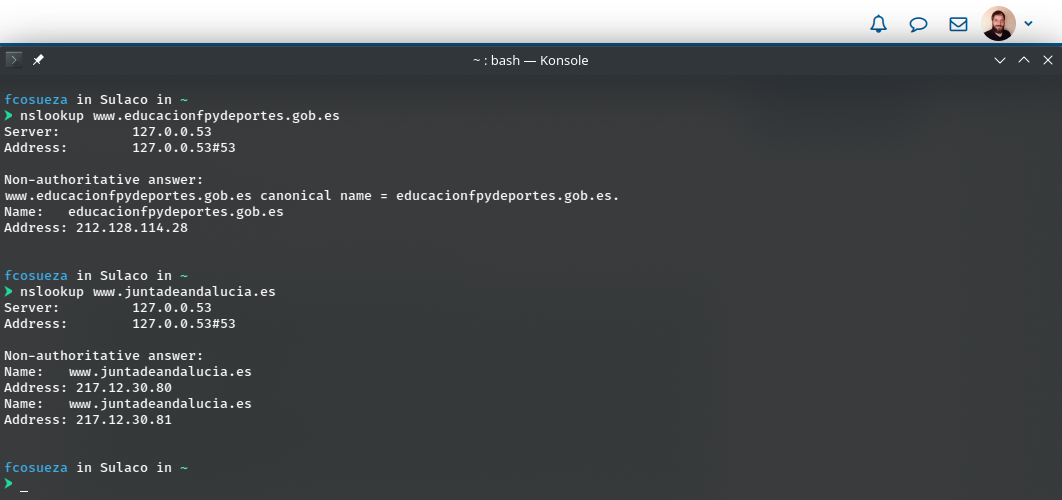
\includegraphics[scale=0.50]{nslook-1.png}
    \caption{Ejecución de nslookup en los dominios especificados}
\end{figure}

\section{Actividad 2: Servidor DNS}

\subsection{Enunciado}
\begin{itemize}
    \item \textbf{Actividad 2.1 - Instalación de bind9}: Realiza la instalación del servicio DNS en Linux (bind9) y configura la interfaz de red para indicarle que el servidor DNS preferido será nuestra propia máquina. Es conveniente (aunque no imprescindible) que configures la interfaz de red como estática. Comprueba que el servicio está funcionando y que el puerto está accesible.

    \item \textbf{Actividad 2.2 - Creación de una zona directa e inversa}: Configura el servidor como un servidor DNS principal y realiza la configuración necesaria para que gestione una zona directa (\textbf{fpad.db}) y una inversa (\textbf{fpad.rev}) para el dominio \textbf{fpad.com}.

    \item \textbf{Actividad 2.3 - Añadiendo registros DNS a las zonas}: Edita los ficheros de zona directa e inversa y crea los registros necesarios para que el servidor resuelva lo siguiente:
    \begin{itemize}
        \item Un servidor web llamado www.fpad.com
        \item Un servidor ftp llamado ftp.fpad.com
        \item Un servidor de correo llamado mail.fpad.com
        \item Un servidor de correo llamado mail.fpad.com
    \end{itemize}

    \item \textbf{Actividad 2.4 Comprobando que los registros funcionan}: Realiza la comprobación de los ficheros de zona con named-checkconf y named-checkzone y realiza la consulta de registros tanto directa como inversa (nslookup, dig,...).
\end{itemize}

\subsection{Solución}
\subsubsection{Instalación de Bind9}
En este ejercicio se va a realizar la instalación de Bind9 y se va a configurar la interfaz de red para que use el servidor instalado como
servidor DNS.

En primer lugar, se ha \textbf{realizado la instalación} del servidor mediante el comando \textbf{APT}, ejecutando el comando \textbf{\textit{apt-get install bind9 bind9utils}}, habiéndose realizado la instalación con éxito como podemos ver en la siguiente captura de pantallas.

\begin{figure}[H]
    \centering
    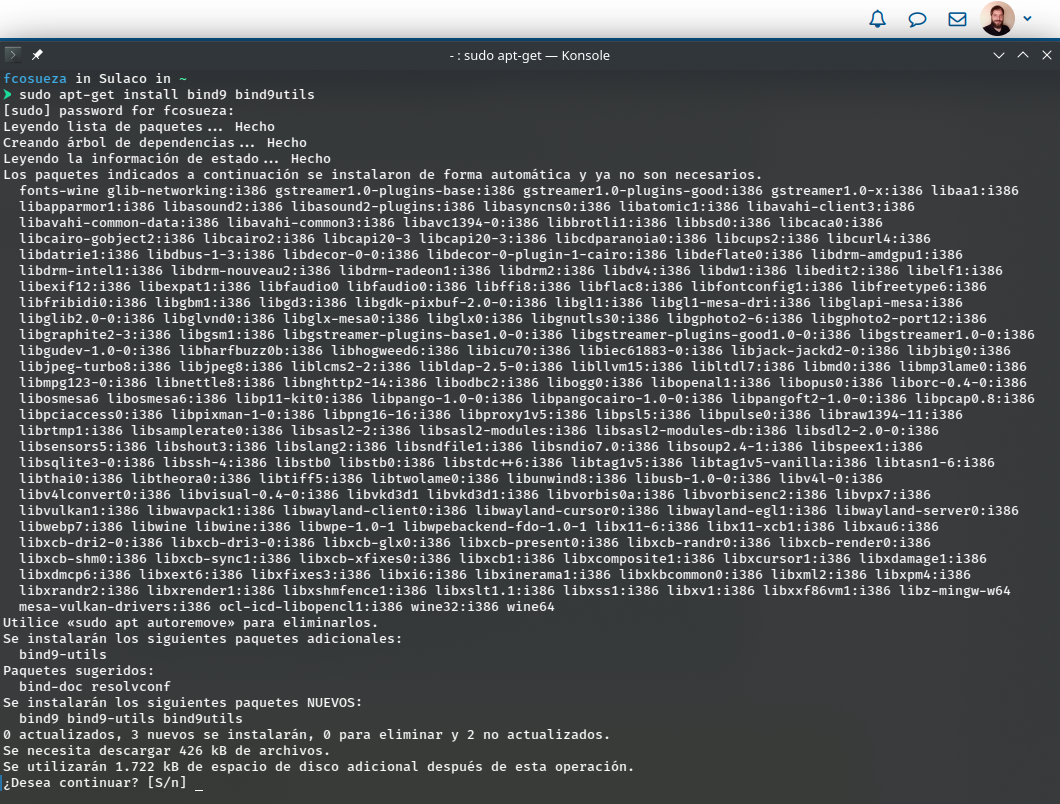
\includegraphics[scale=0.42]{bind-1.png}
    \caption{Instalación de Bind9 con APT}
\end{figure}


Por último, se han realizado las comprobaciones para ver que el servidor se esta ejecutando correctamente y que se esta empleando como DNS principal. Para ello, se han usado los comandos \textbf{nmap}, para que nos indique en que puerto está escuchando el servidor y si esta activo, y el comando \textbf{nslookup} para comprobar que se esta usando el DNS local como DNS principal.

En la siguiente captura podemos ver la ejecución de estos tres comandos y su resultado, comprobando que el servidor se esta ejecutando correctamente y se esta empleando como DNS principal.

\begin{figure}[H]
    \centering
    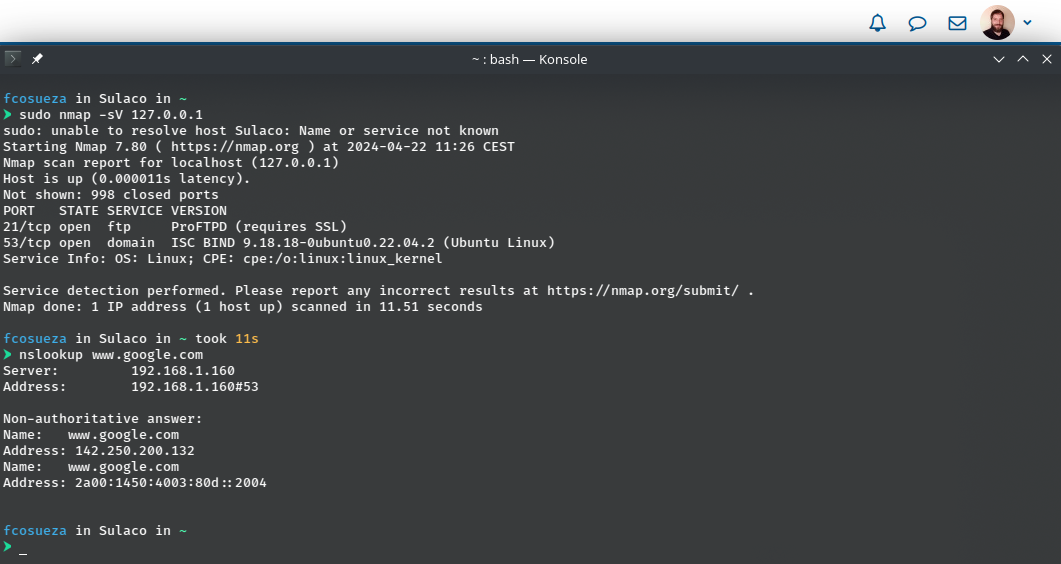
\includegraphics[scale=0.45]{bind-3.png}
    \caption{Comprobación de que el servidor funciona correctamente}
\end{figure}

\subsubsection{Creación de una Zona Directa e Inversa}
En primer lugar, se ha \textbf{configurarado el servidor como DNS princial}, para ello se ha modificado  el archivo \textbf{/etc/resolv.conf}, donde se ha establecido nuestro servidor como servidor DNS predeterminado, como podemos ver en la siguiente captura.

\begin{figure}[H]
    \centering
    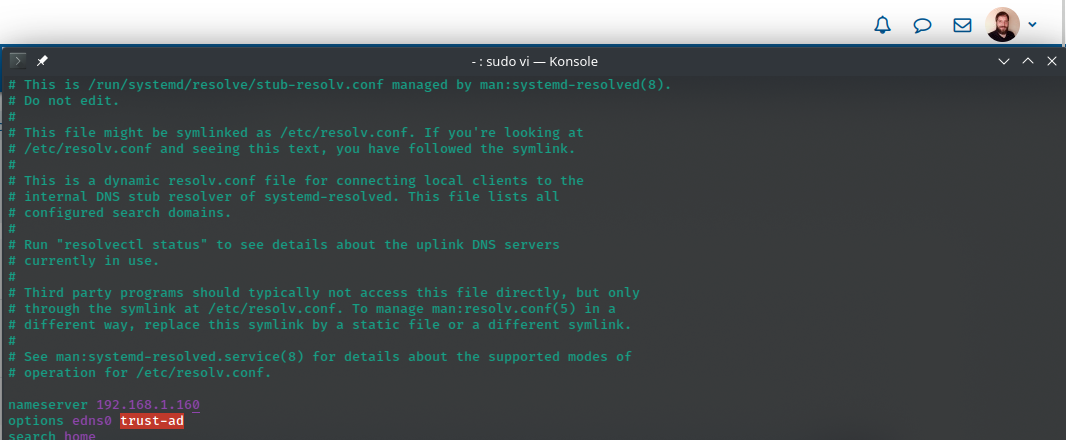
\includegraphics[scale=0.50]{bind-2.png}
    \caption{Estableciendo el servidor local como servidor DNS}
\end{figure}

En siguiente paso ha sido \textbf{añadir dos zonas}, una directa y otra inversa para el dominio \textbf{fpad.com}. Esto se ha llevado a cabo modificando el fichero \textbf{\textit{/etc/bind/named.conf.local}} y añadiendo las opciones adecuadas, las cuales podemos ver con detalle en la siguiente captura.

\begin{figure}[H]
    \centering
    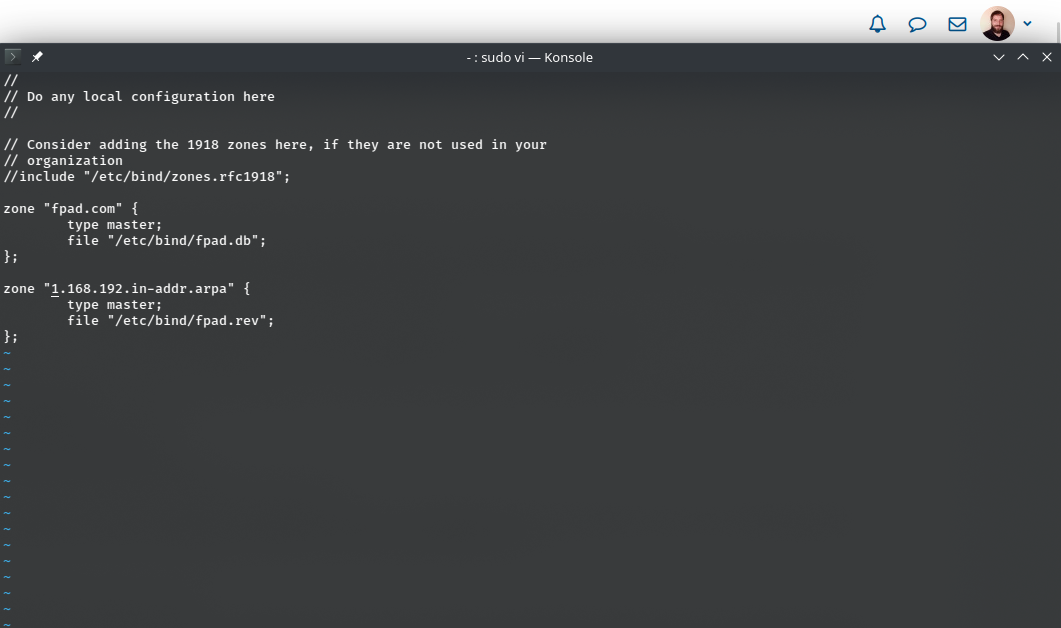
\includegraphics[scale=0.50]{bind-4.png}
    \caption{Creación de la zona directa e inversa}
\end{figure}

\subsubsection{Añadiendo los Registros DNS a las Zonas}
En este siguiente paso vamos a añadir los registros solicitados a las zonas que hemos creado. Esto se va a realizar en los ficheros donde hemos indicado que se almacenará la información de las zonas.

Para configurar estos archivos, se ha cogido como modelo el archivo \textbf{\textit{/etc/bind/db.local}} y se han copiado, modificado y añadido los registros oportunos.

En primer lugar, se ha configurar el archivo de la \textbf{zona directa}, que después de modificar el registro SOA y añadir los diferentes registros que nos pide el enunciado ha quedado como podemos ver en la siguiente captura del \textbf{fichero fpad.db}.

\begin{figure}[H]
    \centering
    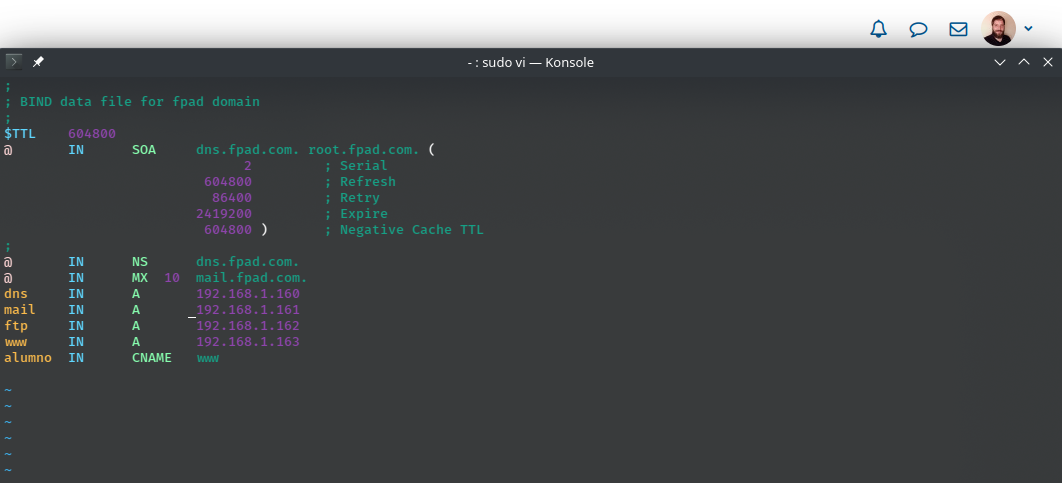
\includegraphics[scale=0.50]{bind-5.png}
    \caption{Registros en la zona directa (fichero fpad.db)}
\end{figure}

El siguiente paso ha sido \textbf{añadir los registros} en la \textbf{zona inversa}. La configuración es bastante similar a la zona reverdad, cambiando los registros por registros tipo PRT y actualizando las IPs. Después de estos cambios, el fichero \textbf{fpad.rev} ha quedado como vemos a continuación.

\begin{figure}[H]
    \centering
    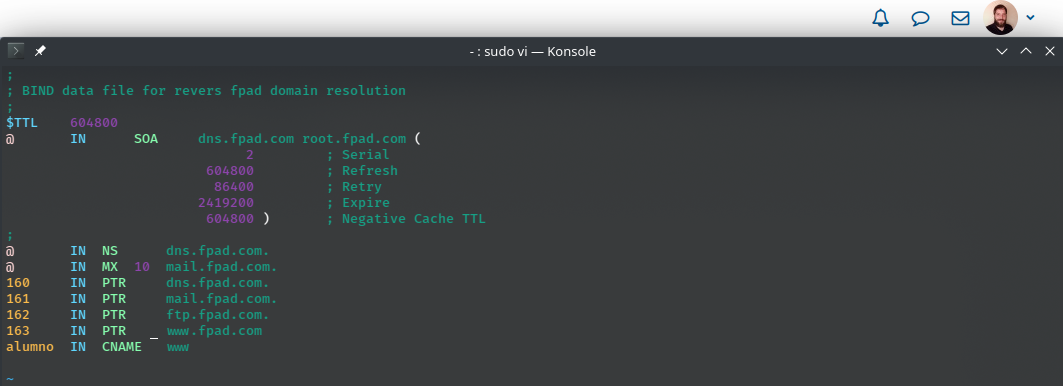
\includegraphics[scale=0.50]{bind-6.png}
    \caption{Registros en la zona reversa (fichero fpad.rev)}
\end{figure}

\subsubsection{Comprobando que los Registros Funcionan}
Una vez realizados los cambios que hemos visto en el punto anterior, vamos a comprobar que éstos funcionan correctamente, para ellos vamos a llevar a cabo 2 pasos en esta comprobación.

En primer lugar, vamos a usar el comando \textbf{name-checkzone} para comprobar que las zonas, tanto del fichero \textbf{fpad.db} como del fichero \textbf{fpad.rev} son correctos. En la siguiente captura, se ha ejecutado esta utilizad para ambos ficheros y como podemos comprobar los dos son correctos.

\begin{figure}[H]
    \centering
    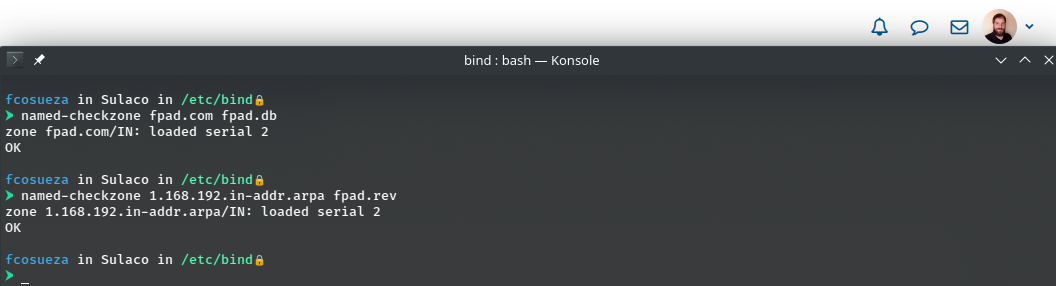
\includegraphics[scale=0.50]{bind-7.png}
    \caption{Comprobación de la corrección de los ficheros fpad.db y fpad.rev}
\end{figure}

A continuación, hemos realizado algunas conversiones con el comando \textbf{nslookup}, tanto directas como reversas, para comprobar que se usa el servidor DNS que hemos configurado y que estas conversiones se realizan de forma correcta. En la siguiente captura, podemos ver varias conversiones con este comando.

\begin{figure}[H]
    \centering
    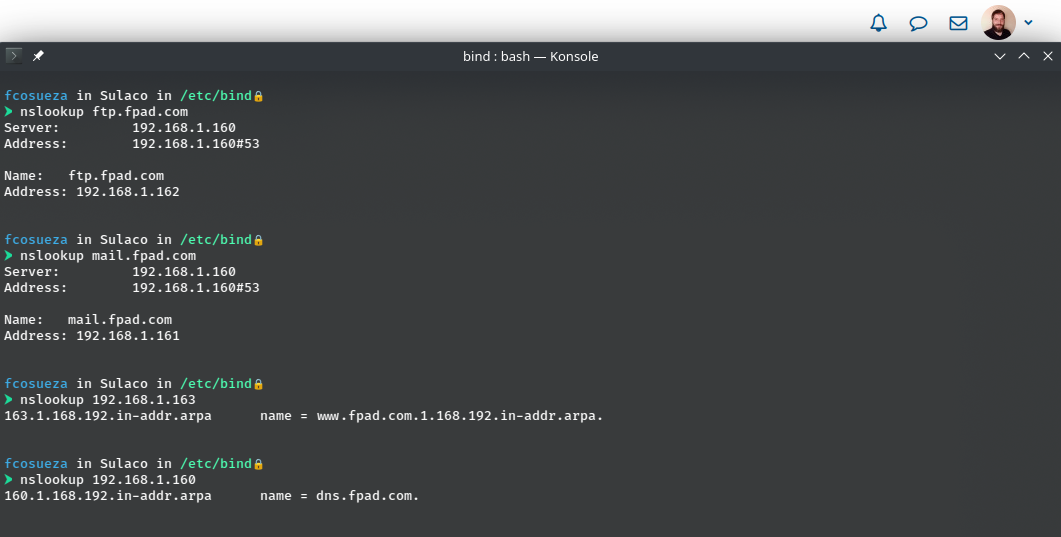
\includegraphics[scale=0.50]{bind-8.png}
    \caption{Comprobación de conversiones con nslookup}
\end{figure}

Como podemos ver, todas las conversiones se han realizado correctamente, por lo que el servidor, así como las zonas que hemos configurado, están funcionando perfectamente.

\section{Actividad 3: Servicio LDAP}
\subsection{Enunciado}
\begin{itemize}
    \item \textbf{Actividad 3.1 - Instalación de LDAP}: Realiza la instalación del servicio de LDAP con OpenLDAP (slapd). Una vez instalado realiza la configuración inicial utilizando como dominio raíz \textbf{distancia24.com} y el password \textbf{distancia}. Realiza una comprobación de la instalación (con slapcat).

    \item \textbf{Actividad 3.2 - Añadir una unidad organizativa a LDAP}: En esta actividad vamos a añadir una unidad organizativa creando un fichero que se llamará uniorg.ldif. Una vez que hayas añadido el contenido correspondiente, añádela al directorio (ldapadd). Comprueba con slapcat.

    \item \textbf{Actividad 3.3 - Añadir un grupo al directorio LDAP}: En esta actividad vamos a añadir un directorio creando un fichero que se llamará group.ldif. Una vez que hayas añadido el contenido correspondiente, añádela al directorio (ldapadd). Realiza una comprobación de los elementos añadidos (slapcat).

    \item \textbf{Actividad 3.4 - Añadir un usuario al directorio LDAP}: Ahora vamos a añadir un usuario, que será la inicial de tu nombre seguida de tu primer apellido, creando un fichero user.ldif. Una vez que hayas añadido el contenido correspondiente, añádela al directorio (ldapadd). Realiza una comprobación de los elementos añadidos (slapcat)
\end{itemize}

\subsection{Solución}
En esta última actividad vamos a instalar y configurar el servicio de directorio \textbf{LDAP} empleando para ello \textbf{OpenLDAP}, una implementación libre y gratuita de este protocolo.

\subsubsection{Instalación de LDAP}
En primer lugar, vamos a realizar la instalación de \textbf{openldap}, empleando para ello el gestor de paquetes \textbf{APT} que usa Kubuntu. En la siguiente captura, podemos ver la ejecución del comando para la instalación de ldap, que incluye los paquetes \textbf{slapd} y \textbf{ldap-utils}.

\begin{figure}[H]
    \centering
    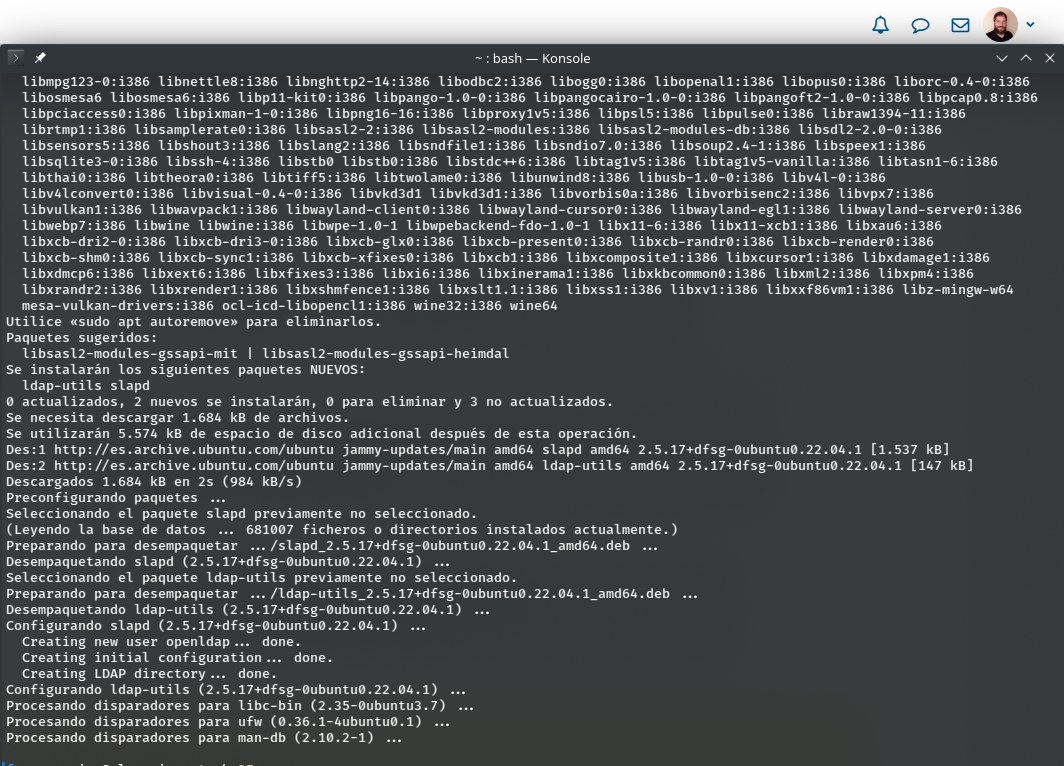
\includegraphics[scale=0.50]{ldap-1.png}
    \caption{Instalación de los paquetes ldap}
\end{figure}

Una vez instalado, vamos a añadir el dominio \textbf{distancia24.com} con la contraseña \textbf{distancia}. Para ello, vamos a usar el comando \textbf{dpkg-reconfigure} para reconfigurar \textbf{slapd}, lo que nos mostrara un menú en ncurses que no irá pidiendo los datos sobre el servidor. En la siguiente captura, podemos ver la introducción del dominio en el menú.

\begin{figure}[H]
    \centering
    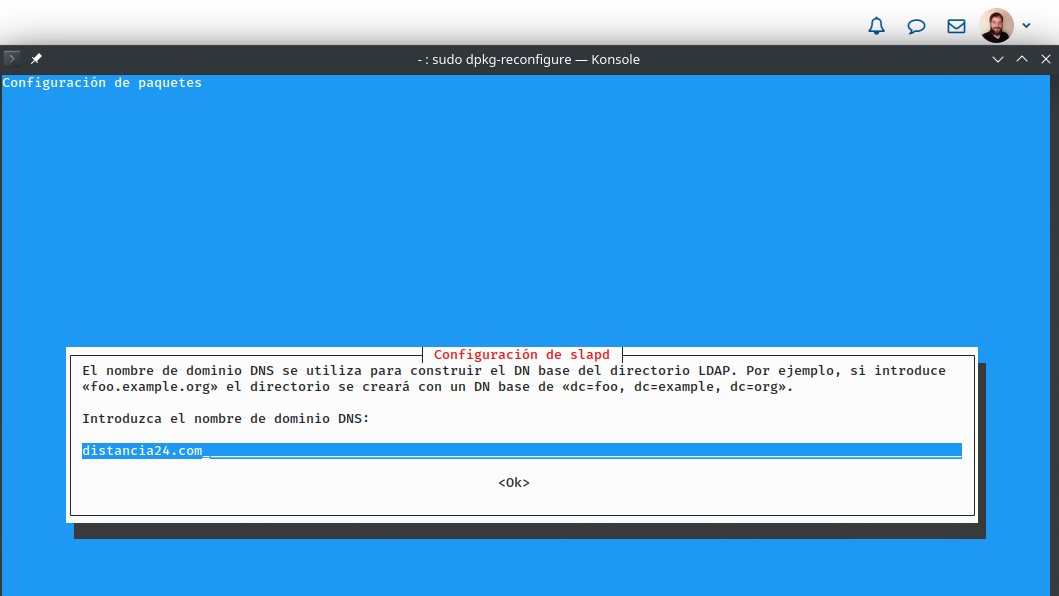
\includegraphics[scale=0.40]{ldap-2.png}
    \caption{Configuración de LDAP}
\end{figure}

Después de rellenar estos datos, la configuración se ha realizado correctamente, pero para asegurarnos, vamos a realizar una comprobación con slapcat, que como vemos en la siguiente captura, nos arroja los datos correctos.

\begin{figure}[H]
    \centering
    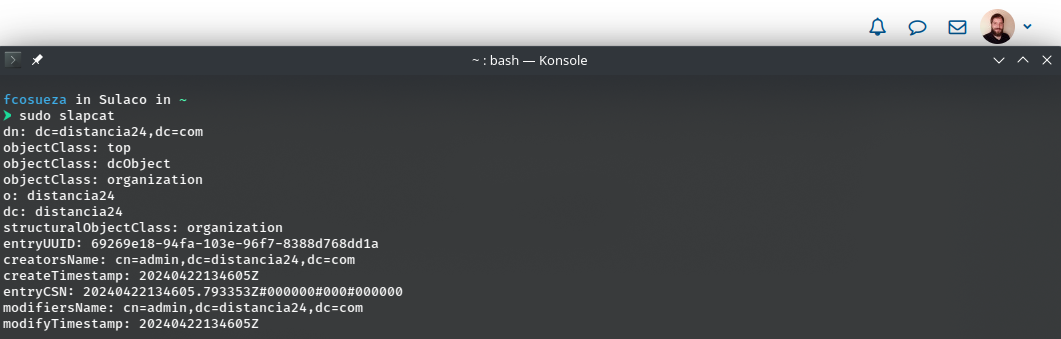
\includegraphics[scale=0.50]{ldap-3.png}
    \caption{Comprobación de las instalación con slapcat}
\end{figure}

Y para comprobar que el servicio esta activo y el puerto esta abierto, hemos utilizad \textbf{nmap}, como hiciéramos anteriormente, que como podemos ver en la siguiente captura, muestras que el servicio esta activo y escuchando en el\textbf{ puerto 389}.

\begin{figure}[H]
    \centering
    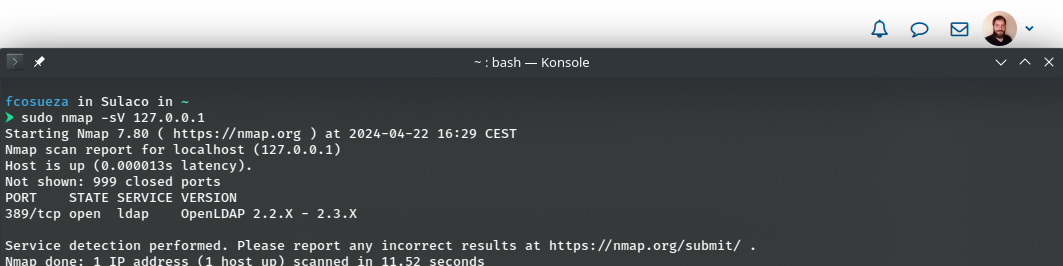
\includegraphics[scale=0.50]{ldap-0.png}
    \caption{Comprobación del puerto con nmap}
\end{figure}


\subsubsection{Añadir Unidad Organizativa al Directorio LDAP}
En primer lugar vamos a añadir una unidad organizativa, creando un el fichero uniorg.ldif, que ha quedado como vemos a continuación.

\begin{figure}[H]
    \centering
    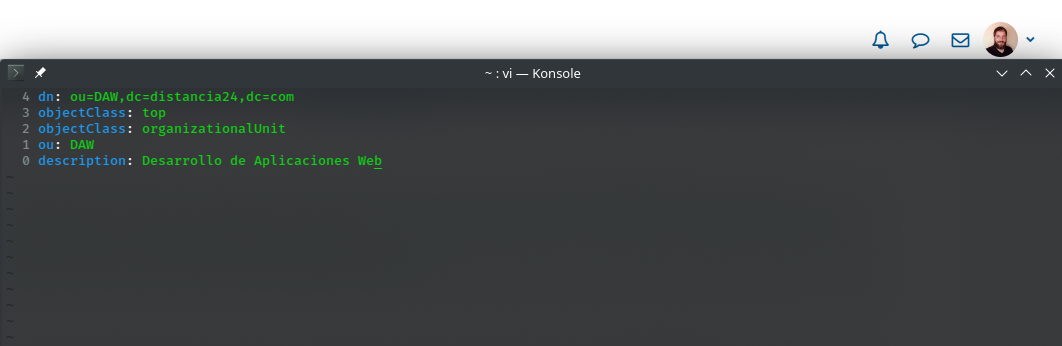
\includegraphics[scale=0.50]{ldap-4.png}
    \caption{Unidad organizativa DAW}
\end{figure}

Como podemos ver, hemos creado una unidad denominada DAW, donde a continuación crearemos grupos usuarios, pero eso será en las siguientes actividades. Ahora mismo, tenemos que añadir la unidad organizativa con el comando \textbf{ldapadd} y comprobar mediante \textbf{slapcat} que se ha añadido correctamente, como podemos ver en la siguiente captura.

\begin{figure}[H]
    \centering
    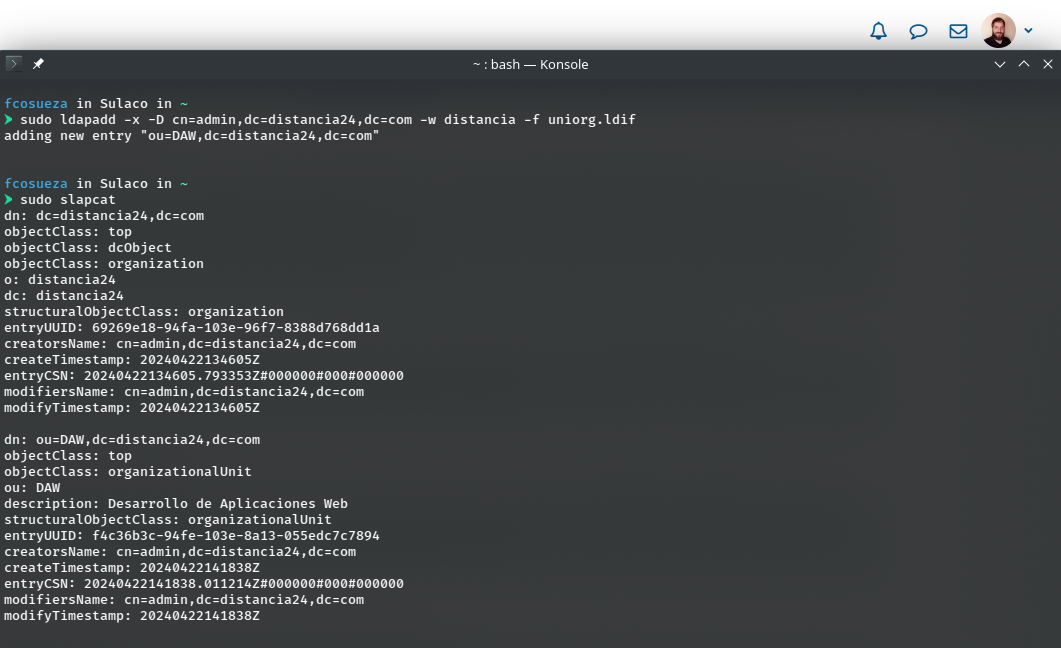
\includegraphics[scale=0.50]{ldap-5.png}
    \caption{Inserción de la unidad organizativa y comprobación}
\end{figure}

\subsubsection{Creación de un Grupo en el Directorio LDAP}
En este apartado vamos a \textbf{añadir un grupo} al directorio LDAP. Lo vamos a hacer dentro de la unidad organizativa que hemos creado en el punto anterior y se va a llamar \textbf{despliegue}, donde almacenaremos información sobre esta asignatura.

Para añadir un grupo, se ha creado el fichero \textbf{grupo.ldif} y se han introducido los datos adecuados, quedando el fichero como podemos ver en la siguiente imagen.


\begin{figure}[H]
    \centering
    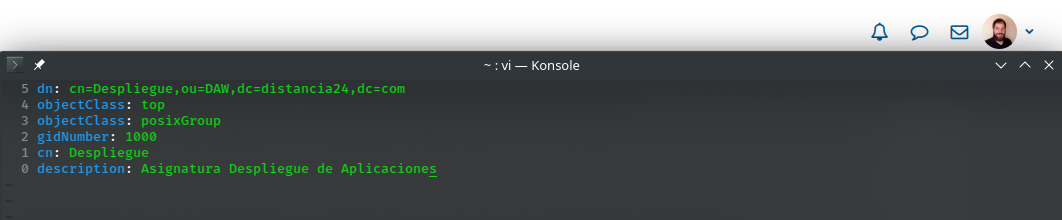
\includegraphics[scale=0.50]{ldap-6.png}
    \caption{Fichero grupo.ldif}
\end{figure}

Una vez creado el fichero, hemos realizado el mismo paso que en el punto anterior, añadiendo la información al directorio con el comando \textbf{ldapadd} y comprobando que se ha realizado correctamente con \textbf{slapcat}, como vemos a continuación.

\begin{figure}[H]
    \centering
    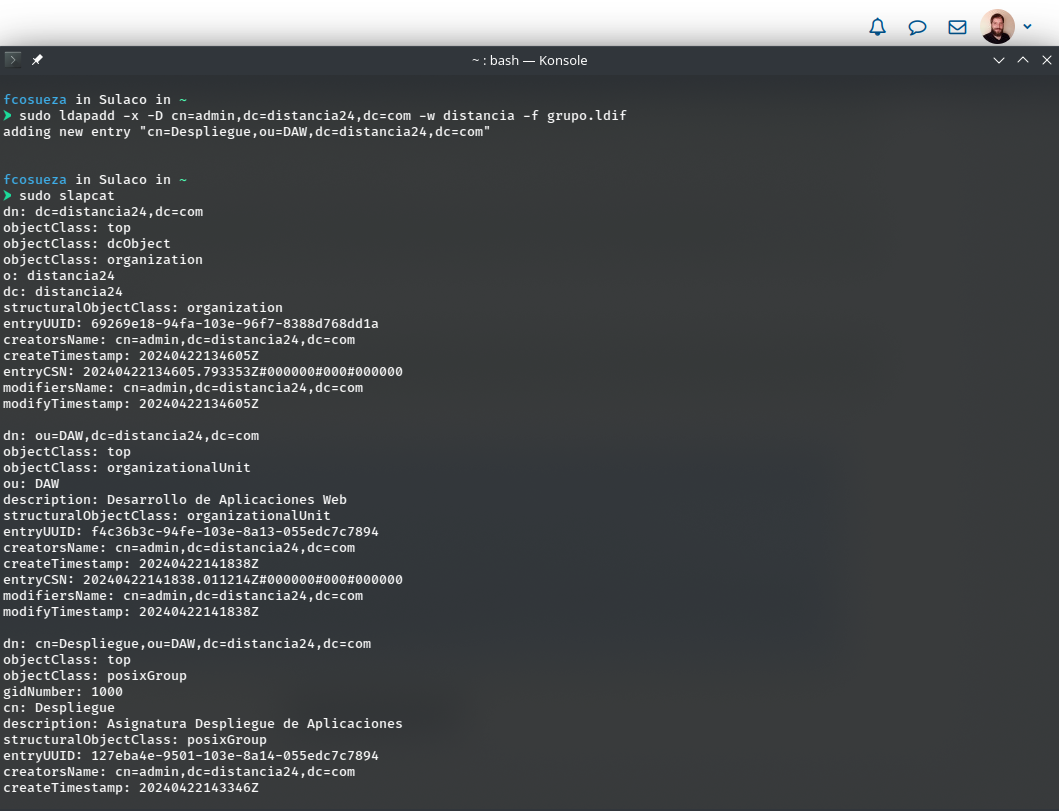
\includegraphics[scale=0.50]{ldap-7.png}
    \caption{Inserción del grupo en el directorio y comprobación}
\end{figure}

\subsubsection{Añadir un Usuario al Directorio LDAP}
Por último, vamos a añadir un usuario al directorio. Para ello hemos creado el fichero \textbf{user.ldif} e introducido los datos en el, quedando como se puede ver en la siguiente captura.

\begin{figure}[H]
    \centering
    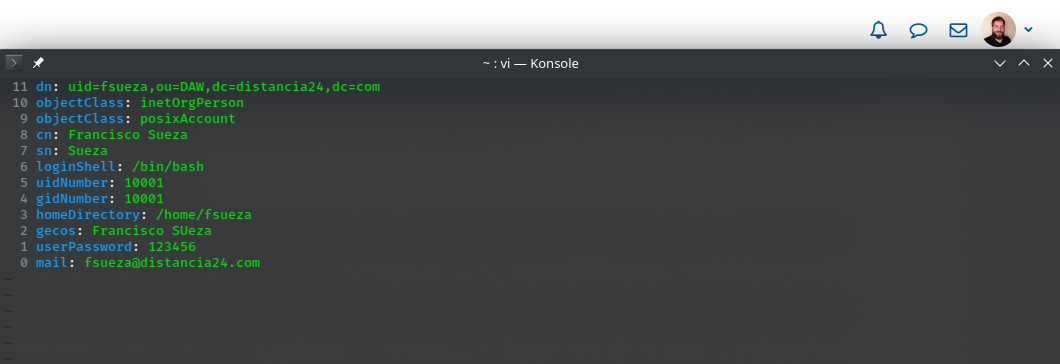
\includegraphics[scale=0.50]{ldap-8.png}
    \caption{Fichero user.ldif}
\end{figure}

Por último, lo hemos añadido y hemos verificado que se ha añadido correctamente, como podemos ver en la siguiente captura con la ejecución del comando \textbf{slapcat}.

\begin{figure}[H]
    \centering
    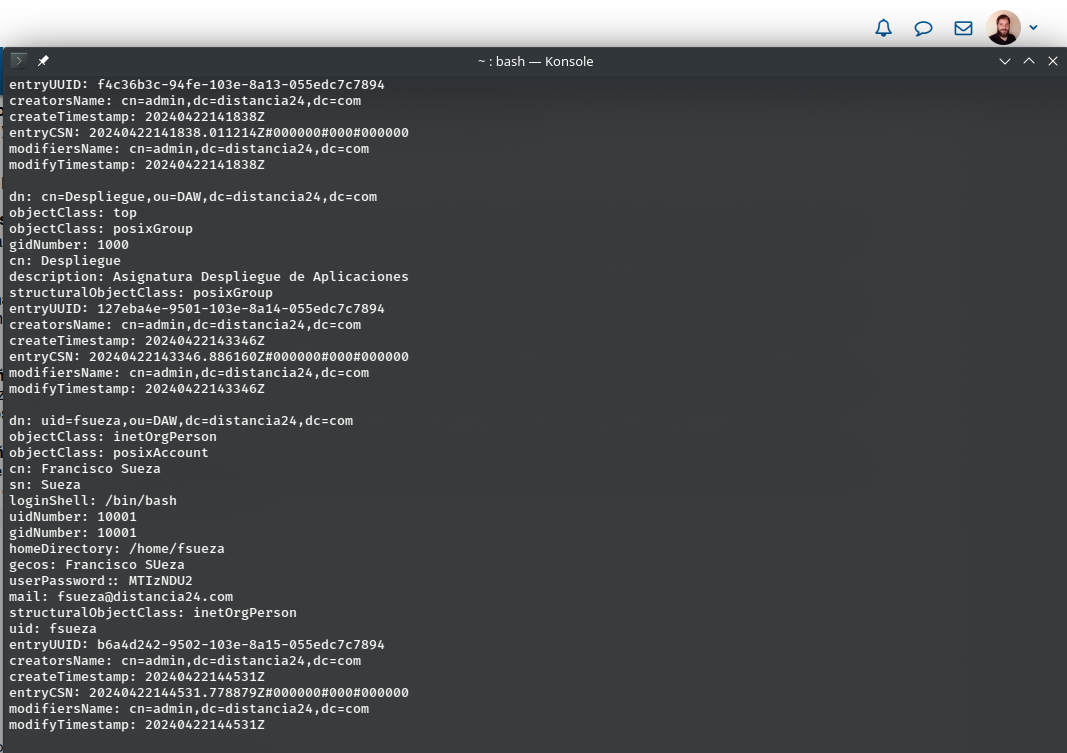
\includegraphics[scale=0.50]{ldap-9.png}
    \caption{Inserción del usuario en el directorio y comprobación}
\end{figure}
% Bibliography

%\newpage
%\bibliography{citas}
%\bibliographystyle{unsrt}

\end{document}